\section{Phase 1 - Uniform Bonding}

\subsection{Characterization of Indium Bonding Spread}
After a repeatable electroplating process for indium was developed, the next step was to investigate how the indium would spread once die-bonded. The spreading behaviour of indium is critical because it can impact the performance of the semiconductor device. Specifically, the spreading of indium can affect the heat dissipation and the electrical contact between the die and the substrate. Understanding this behaviour is essential for optimizing the performance of the device.
This knowledge can then be used to inform the design and manufacture of semiconductor devices, improving their reliability and performance.
Diebonding is the process of placing a semiconductor chip onto a substrate or package, and eutectic bonding is a common diebonding technique. Understanding the behaviour of indium during eutectic bonding is crucial for ensuring the reliability and performance of the final device.

\begin{table}[ht]
    \begingroup
    \renewcommand{\minval}{2.61}
    \renewcommand{\maxval}{18.1}
    \scriptsize
    \centering
    \begin{center}
        \begin{tabular}{*{12}{|m{0.7cm}}|}
            \hline
            \grd{4.80}  &   & \grd{5.22}    &               &   & \grd{3.98}    & \grd{4.05}    &   &               & \grd{5.32}    &   & \grd{5.33}    \\[0.7cm]\hline
                        &   &               &               &   &               &               &   &               &               &   &               \\[0.7cm]\hline
                        &   &               &               &   & \grd{3.33}    & \grd{4.85}    &   &               &               &   &               \\[0.7cm]\hline
            \grd{2.61}  &   &               & \grd{3.18}    &   &               &               &   & \grd{4.81}    &               &   & \grd{5.40}    \\[0.7cm]\hline
                        &   &               &               &   &               &               &   &               &               &   &               \\[0.7cm]\hline
            \grd{3.02}  &   & \grd{3.11}    &               &   & \grd{3.88}    & \grd{5.29}    &   &               & \grd{3.78}    &   & \grd{3.88}    \\[0.7cm]\hline
            \grd{6.55}  &   & \grd{12.0}    &               &   & \grd{18.1}    & \grd{4.94}    &   &               & \grd{4.55}    &   & \grd{5.01}    \\[0.7cm]\hline
                        &   &               &               &   &               &               &   &               &               &   &               \\[0.7cm]\hline
            \grd{6.15}  &   &               & \grd{6.28}    &   & \grd{8.82}    &               &   &               &               &   & \grd{6.04}    \\[0.7cm]\hline
                        &   &               &               &   &               & \grd{4.95}    &   &               & \grd{4.67}    &   &               \\[0.7cm]\hline
                        &   &               &               &   &               &               &   &               &               &   &               \\[0.7cm]\hline
            \grd{6.21}  &   & \grd{11.1}    &               &   & \grd{8.57}    & \grd{5.08}    &   &               & \grd{5.54}    &   & \grd{5.99}    \\[0.7cm]\hline
        \end{tabular}
    \end{center}
    \endgroup
    \caption{Indium bump height map}
\end{table}


\begin{table}[ht]
    \begingroup
    \renewcommand{\minval}{14.9}
    \renewcommand{\maxval}{25.6}
    \scriptsize
    \centering
    \begin{center}
        \begin{tabular}{*{12}{|m{0.7cm}}|}
            \hline
            \grd{16.4}  &   & \grd{18.7}    &               &   & \grd{16.5}    & \grd{16.1}    &   &               & \grd{16.5}    &   & \grd{16.0}    \\[0.7cm]\hline
                        &   &               &               &   &               &               &   &               &               &   &               \\[0.7cm]\hline
                        &   &               &               &   & \grd{16.1}    & \grd{16.0}    &   &               &               &   &               \\[0.7cm]\hline
            \grd{17.1}  &   &               & \grd{16.3}    &   &               &               &   & \grd{15.4}    &               &   & \grd{15.9}    \\[0.7cm]\hline
                        &   &               &               &   &               &               &   &               &               &   &               \\[0.7cm]\hline
            \grd{17.0}  &   & \grd{16.7}    &               &   & \grd{15.6}    & \grd{16.3}    &   &               & \grd{15.4}    &   & \grd{15.8}    \\[0.7cm]\hline
            \grd{14.9}  &   & \grd{21.8}    &               &   & \grd{25.6}    & \grd{18.0}    &   &               & \grd{19.5}    &   & \grd{17.6}    \\[0.7cm]\hline
                        &   &               &               &   &               &               &   &               &               &   &               \\[0.7cm]\hline
            \grd{19.7}  &   &               & \grd{19.3}    &   & \grd{20.8}    &               &   &               &               &   & \grd{19.7}    \\[0.7cm]\hline
                        &   &               &               &   &               & \grd{18.7}    &   &               & \grd{19.5}    &   &               \\[0.7cm]\hline
                        &   &               &               &   &               &               &   &               &               &   &               \\[0.7cm]\hline
            \grd{20.4}  &   & \grd{21.8}    &               &   & \grd{17.2}    & \grd{20.1}    &   &               & \grd{22.2}    &   & \grd{21.4}    \\[0.7cm]\hline
        \end{tabular}
    \end{center}
    \endgroup
    \caption{Indium bump width map}
\end{table}

\begin{table}[ht]
    \begingroup
    \renewcommand{\minval}{000}
    \renewcommand{\maxval}{9316}
    \scriptsize
    \centering
    \begin{center}
        \begin{tabular}{*{12}{|m{0.7cm}}|}
            \hline
            \grd{1014}  &   & \grd{1434}    &               &   & \grd{ 851}        & \grd{ 819}        &   &               & \grd{1131}        &   & \grd{1072}        \\[0.7cm]\hline
                        &   &               &               &   &                   &                   &   &               &                   &   &                   \\[0.7cm]\hline
                        &   &               &               &   & \grd{ 678}        & \grd{ 975}        &   &               &                   &   &                   \\[0.7cm]\hline
            \grd{ 599}  &   &               & \grd{ 664}    &   &                   &                   &   & \grd{ 896}    &                   &   & \grd{1065}        \\[0.7cm]\hline
                        &   &               &               &   &                   &                   &   &               &                   &   &                   \\[0.7cm]\hline
            \grd{ 685}  &   & \grd{ 681}    &               &   & \grd{ 742}        & \grd{1097}        &   &               & \grd{ 704}        &   & \grd{ 761}        \\[0.7cm]\hline
            \grd{1142}  &   & \grd{4479}    &               &   & \grd{9316}        & \grd{1257}        &   &               & \grd{1352}        &   & \grd{1212}        \\[0.7cm]\hline
                        &   &               &               &   &                   &                   &   &               &                   &   &                   \\[0.7cm]\hline
            \grd{1875}  &   &               & \grd{1828}    &   & \grd{2995}        &                   &   &               &                   &   & \grd{1832}        \\[0.7cm]\hline
                        &   &               &               &   &                   & \grd{1359}        &   &               & \grd{1395}        &   &                   \\[0.7cm]\hline
                        &   &               &               &   &                   &                   &   &               &                   &   &                   \\[0.7cm]\hline
            \grd{2030}  &   & \grd{4145}    &               &   & \grd{1979}        & \grd{1604}        &   &               & \grd{2135}        &   & \grd{2144}        \\[0.7cm]\hline
        \end{tabular}
    \end{center}
    \endgroup
    \caption{Indium bump volume map}
\end{table}

A flipchip diebonder is a machine that is used to bond microelectronic chips directly onto a substrate. It allows for precise alignment and bonding of the chip to the substrate, which is essential for the proper functioning of microelectronic devices. In addition to the standard bonding techniques, a flipchip diebonder with eutectic bonding capabilities enables the bonding of two chips by bonding with precise control of heat and pressure, which can greatly enhance the reliability and performance of the microelectronic device. Eutectic bonding is a specialized technique that involves heating the two materials to their eutectic point, at which they melt and fuse together, creating a strong and reliable bond. This makes the flipchip diebonder with eutectic bonding capability a valuable tool in the field of microelectronics for high-performance and reliable bonding of chips to substrates.


The diebonder being used is the `TRESKY-diebond' tool in the QNC packaging lab it is the Tresky T-3000-FC3 model.
The tool is capable of providing a bonding force of up to $490 \unit{\newton}$ ($50 \unit{\kg}$ mass) may be applied at temperatures up to $400 \dC$. The datasheet suggests that it offers placement accuracy of $10\um$ \cite{diebonderDatasheet}.

The current process of diebonding is


Since we want to calculate and understand how the indium will conform when bonding is done, a number of characterization measurements were conducted to understand how the indium will spread and expand over the sample surface.

Since the volume of indium will not change when diebonding occurs, we can model the spread of indium as a flattening of a cylinder.

\begin{equation}\tag{B}
    \begin{split}
        V_{Cylinder Initial} &= V_{Cylinder Final} \\
        \pi \times r_{Initial}^2 \times h_{Initial} &= \pi \times r_{Final}^2 \times h_{Final} \\
        \sqrt{\frac{h_{Initial}}{h_{Final}}} r_{Initial} &= r_{Final} \\
        \sqrt{\frac{h_{Initial}}{ 0.65 \um}} r_{Initial} &= r_{Final}
    \end{split}
\end{equation}



\begin{wrapfigure}{L}{0.7\textwidth}
    \centering
    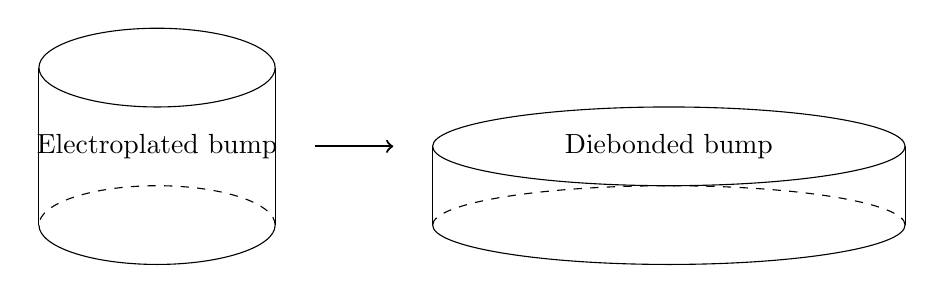
\begin{tikzpicture}
        % First cylinder
        \draw           (   0,   0) ellipse (1.5 and 0.5); % top
        \draw[dashed]   ( 1.5,  -2) arc     (  0:180:1.5 and 0.5); % base
        \draw           (-1.5,  -2) arc     (180:360:1.5 and 0.5); % base
        \draw           (-1.5,  -2) --      (-1.5, 0);
        \draw           ( 1.5,  -2) --      ( 1.5, 0);

        % Second cylinder
        \draw           (1.5+5,  -1) ellipse (3 and 0.5); % top
        \draw[dashed]   (1.5+8,  -2) arc     (  0:180:3 and 0.5); % base
        \draw           (1.5+2,  -2) arc     (180:360:3 and 0.5); % base
        \draw           (1.5+2,  -1) --      (1.5+2, -2);
        \draw           (1.5+8,  -1) --      (1.5+8, -2);

        % Labels
        \node at        (  0 ,  -1) {Electroplated bump};
        \node at        (1.5+5, -1) {Diebonded bump};

        \draw [->,thick](   2,  -1) ->       (3, -1);
        \end{tikzpicture}
    \caption{Line drawing of the change in shape of indium shape (not to scale).}
\end{wrapfigure}


Based on a number of bonding experiments I determined that the average thickness of indium after bonding was around $65 \um$ a sample of the indium bump can be seen in figure \ref{fig:semIndium}

\begin{figure}
    \centering
    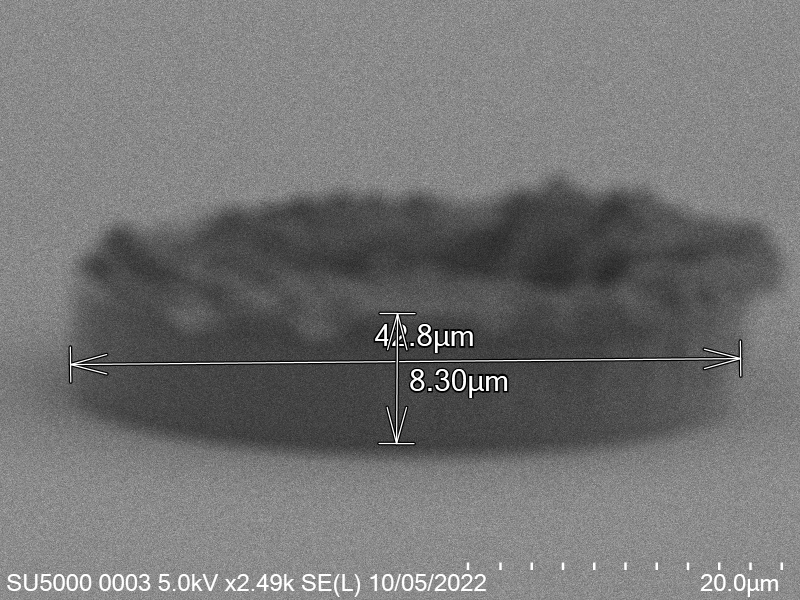
\includegraphics[width=0.65\textwidth]{Main/Ch2/indium_bump_before_bond.png}
    \caption{SEM image of indium bump at an angle of $80^\circ$}
    \label{fig:semIndium}
\end{figure}

The raw data from which I determined the average indium thickness is from table \ref{table:thicknessMap}.

\begin{sidewaystable}
    \centering
    \renewcommand{\minval}{0.1}
    \renewcommand{\maxval}{3}
    \begin{tabular}{| l | c | c | c | c | c|}
    \hline
    Bond ID  &  In Bond Avg. Diameter ($\um$)  &  Indium Thickness ($\um$)  &  In Bump Width ($\um$)  &  In Bump Volume ($\um^3$)  &  Bond Estimated Thickness ($\um$)
    \\
    \hline
    \hline
    BID-005  &  58.6  & 1.3   & 42 & 1801   & \grd{0.667} \\
    BID-006  &  84    & 1.7   & 42 & 2355   & \grd{0.425} \\
    BID-008  &  200   & 14    & 42 & 19396  & \grd{0.617} \\
    BID-009  &  86    & 8.4   & 42 & 11637  & \grd{2.003} \\
    BID-010  &  105   & 8.3   & 42 & 11499  & \grd{1.328} \\
    BID-011  &  142   & 8.5   & 42 & 11776  & \grd{0.743} \\
    BID-012  &  164   & 10    & 42 & 13854  & \grd{0.655} \\
    \hline
    \hline
    \end{tabular}
    \caption{Table of estimated thickness post diebonding}
    \label{table:thicknessMap}
\end{sidewaystable}

From the table after removing outlier values, the median resulting thickness is $ ~65 \um $.

The spread values were identified from images taken from the microscope `OLYMPUS-scope3' in the packaging lab.

From the images captured by the scope \ref{fig:microscopeIndium}, we can see that the gimble head in the lab provides sufficiently uniform bonding pressure over the bonding area. The images also show that there is spreading of the indium as the bond is formed directly as a function of the indium volume.

Knowing that the bond does spread will constrain the maximum density of \uleds \ for a given bump thickness.

\begin{wrapfigure}{R}{0.5\textwidth}
    \centering
    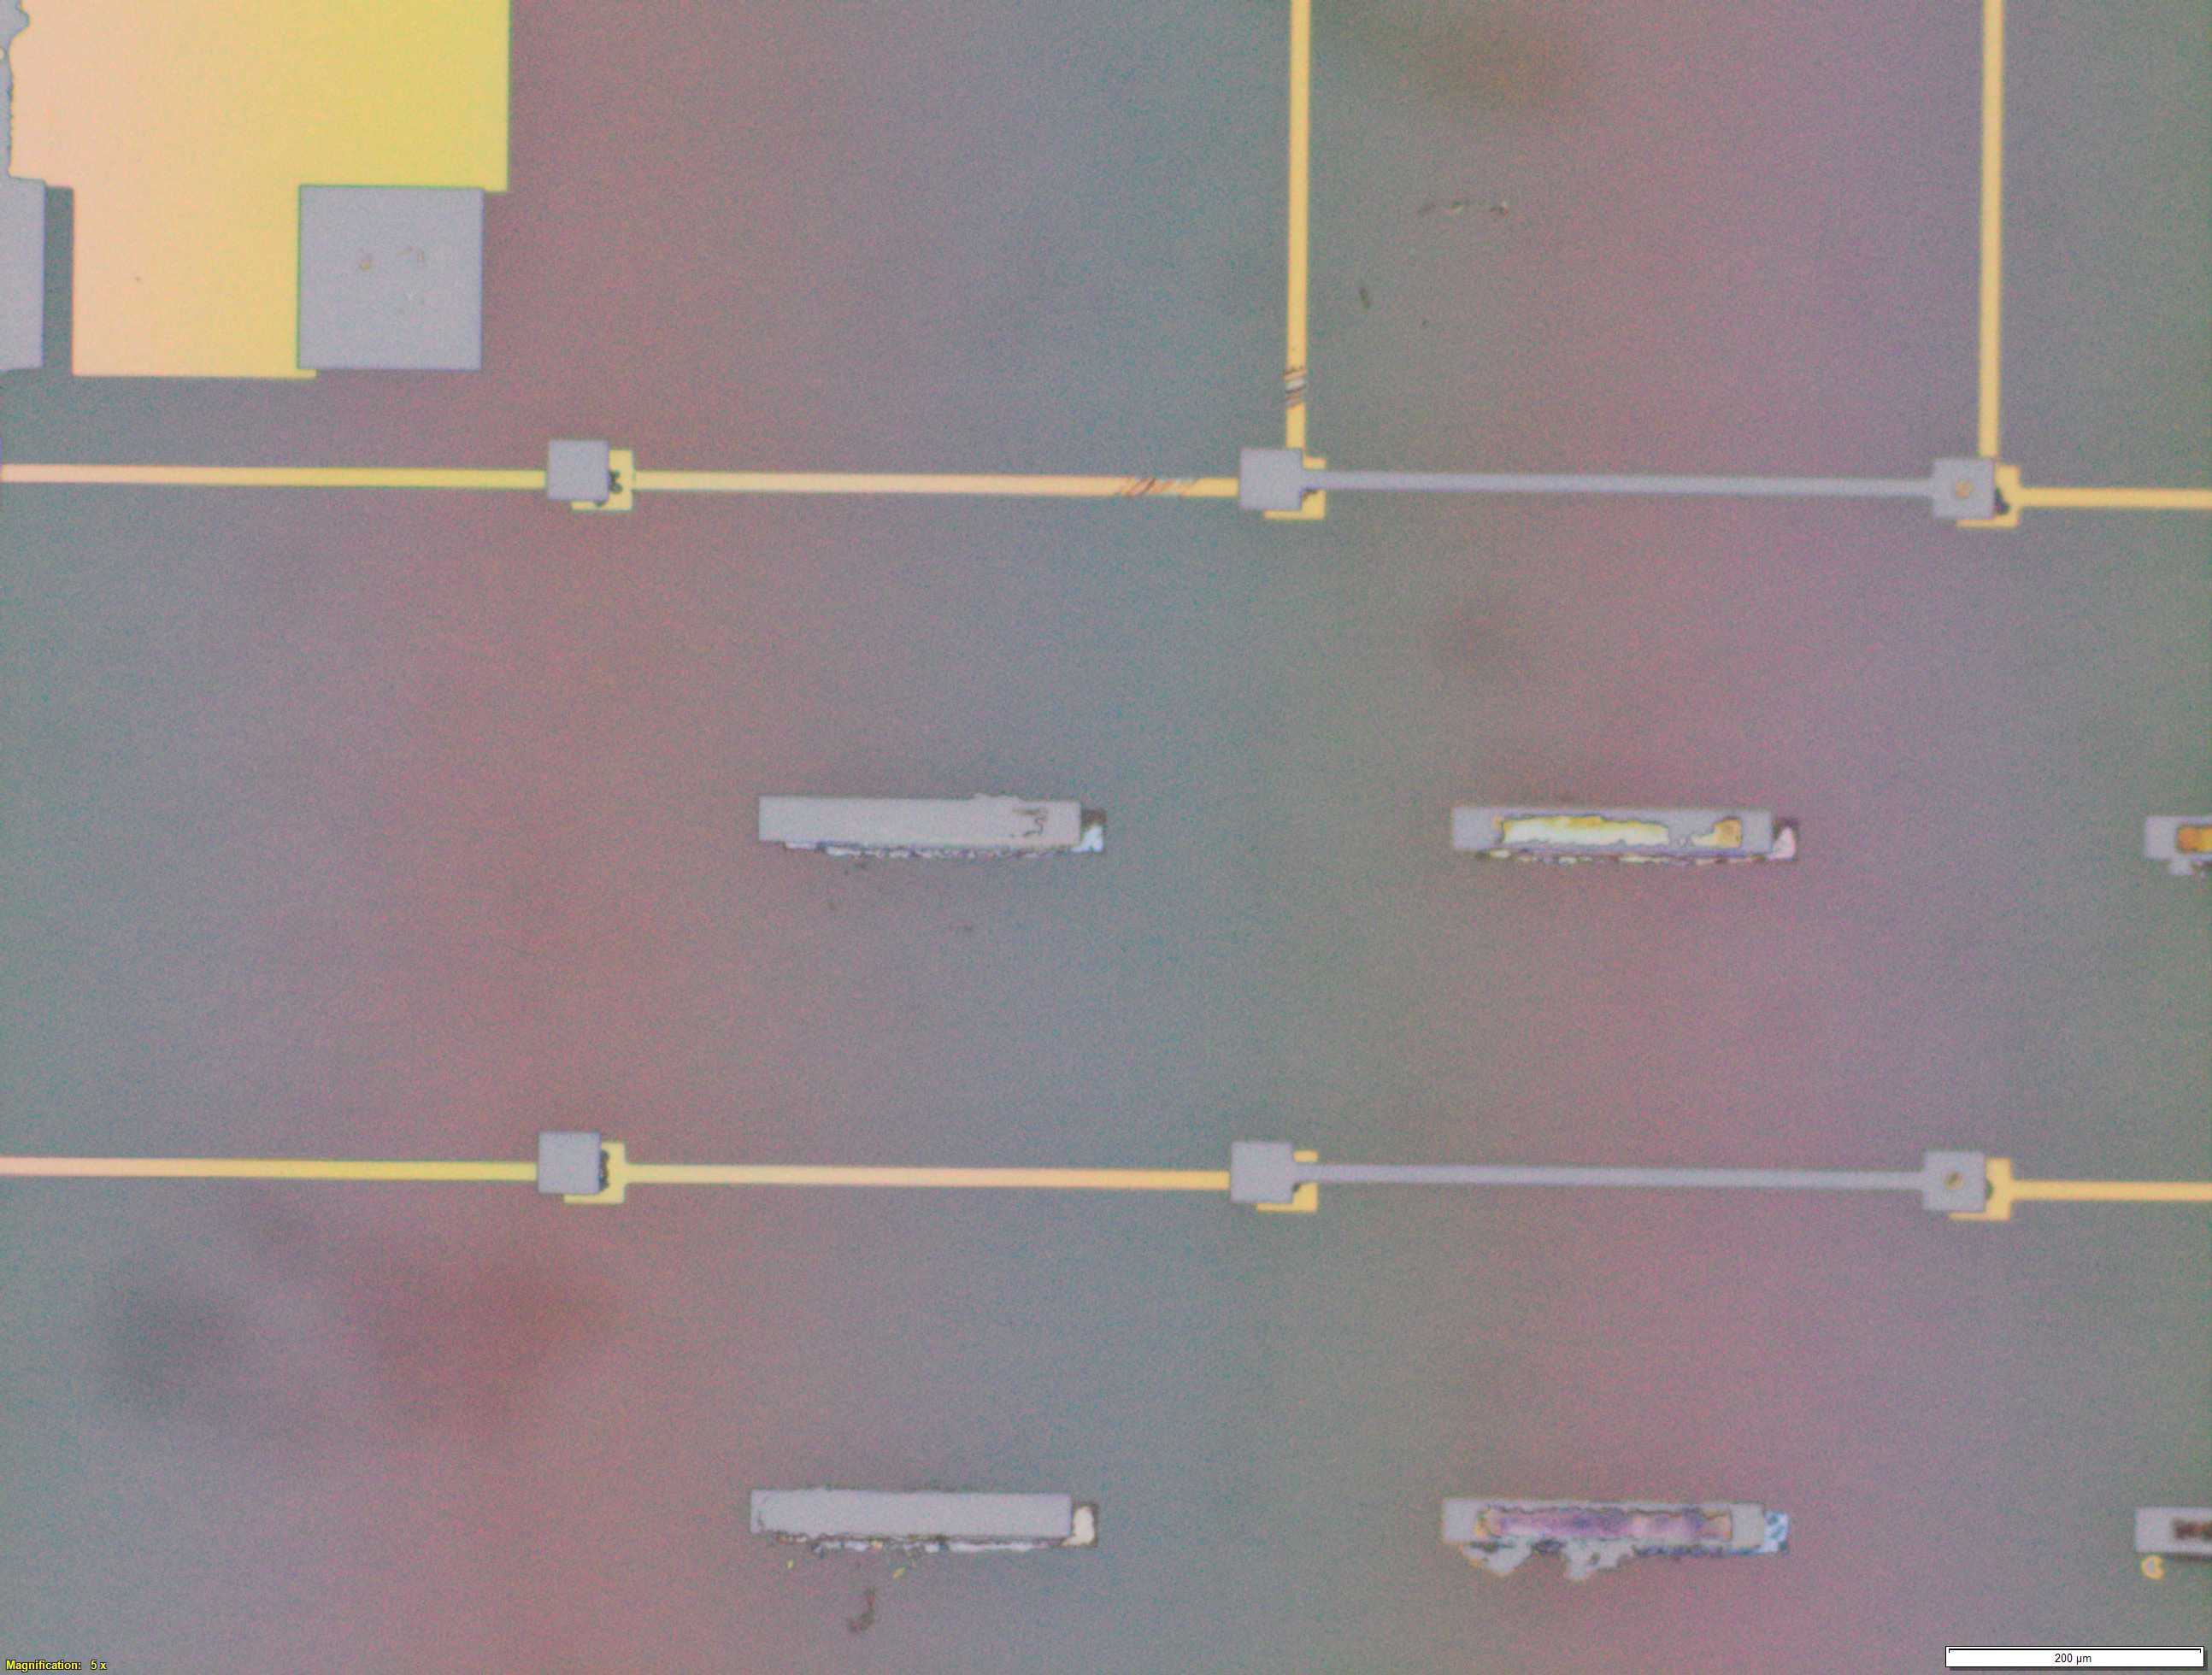
\includegraphics[width=0.22\textwidth]{Main/Ch2/TL.png}
    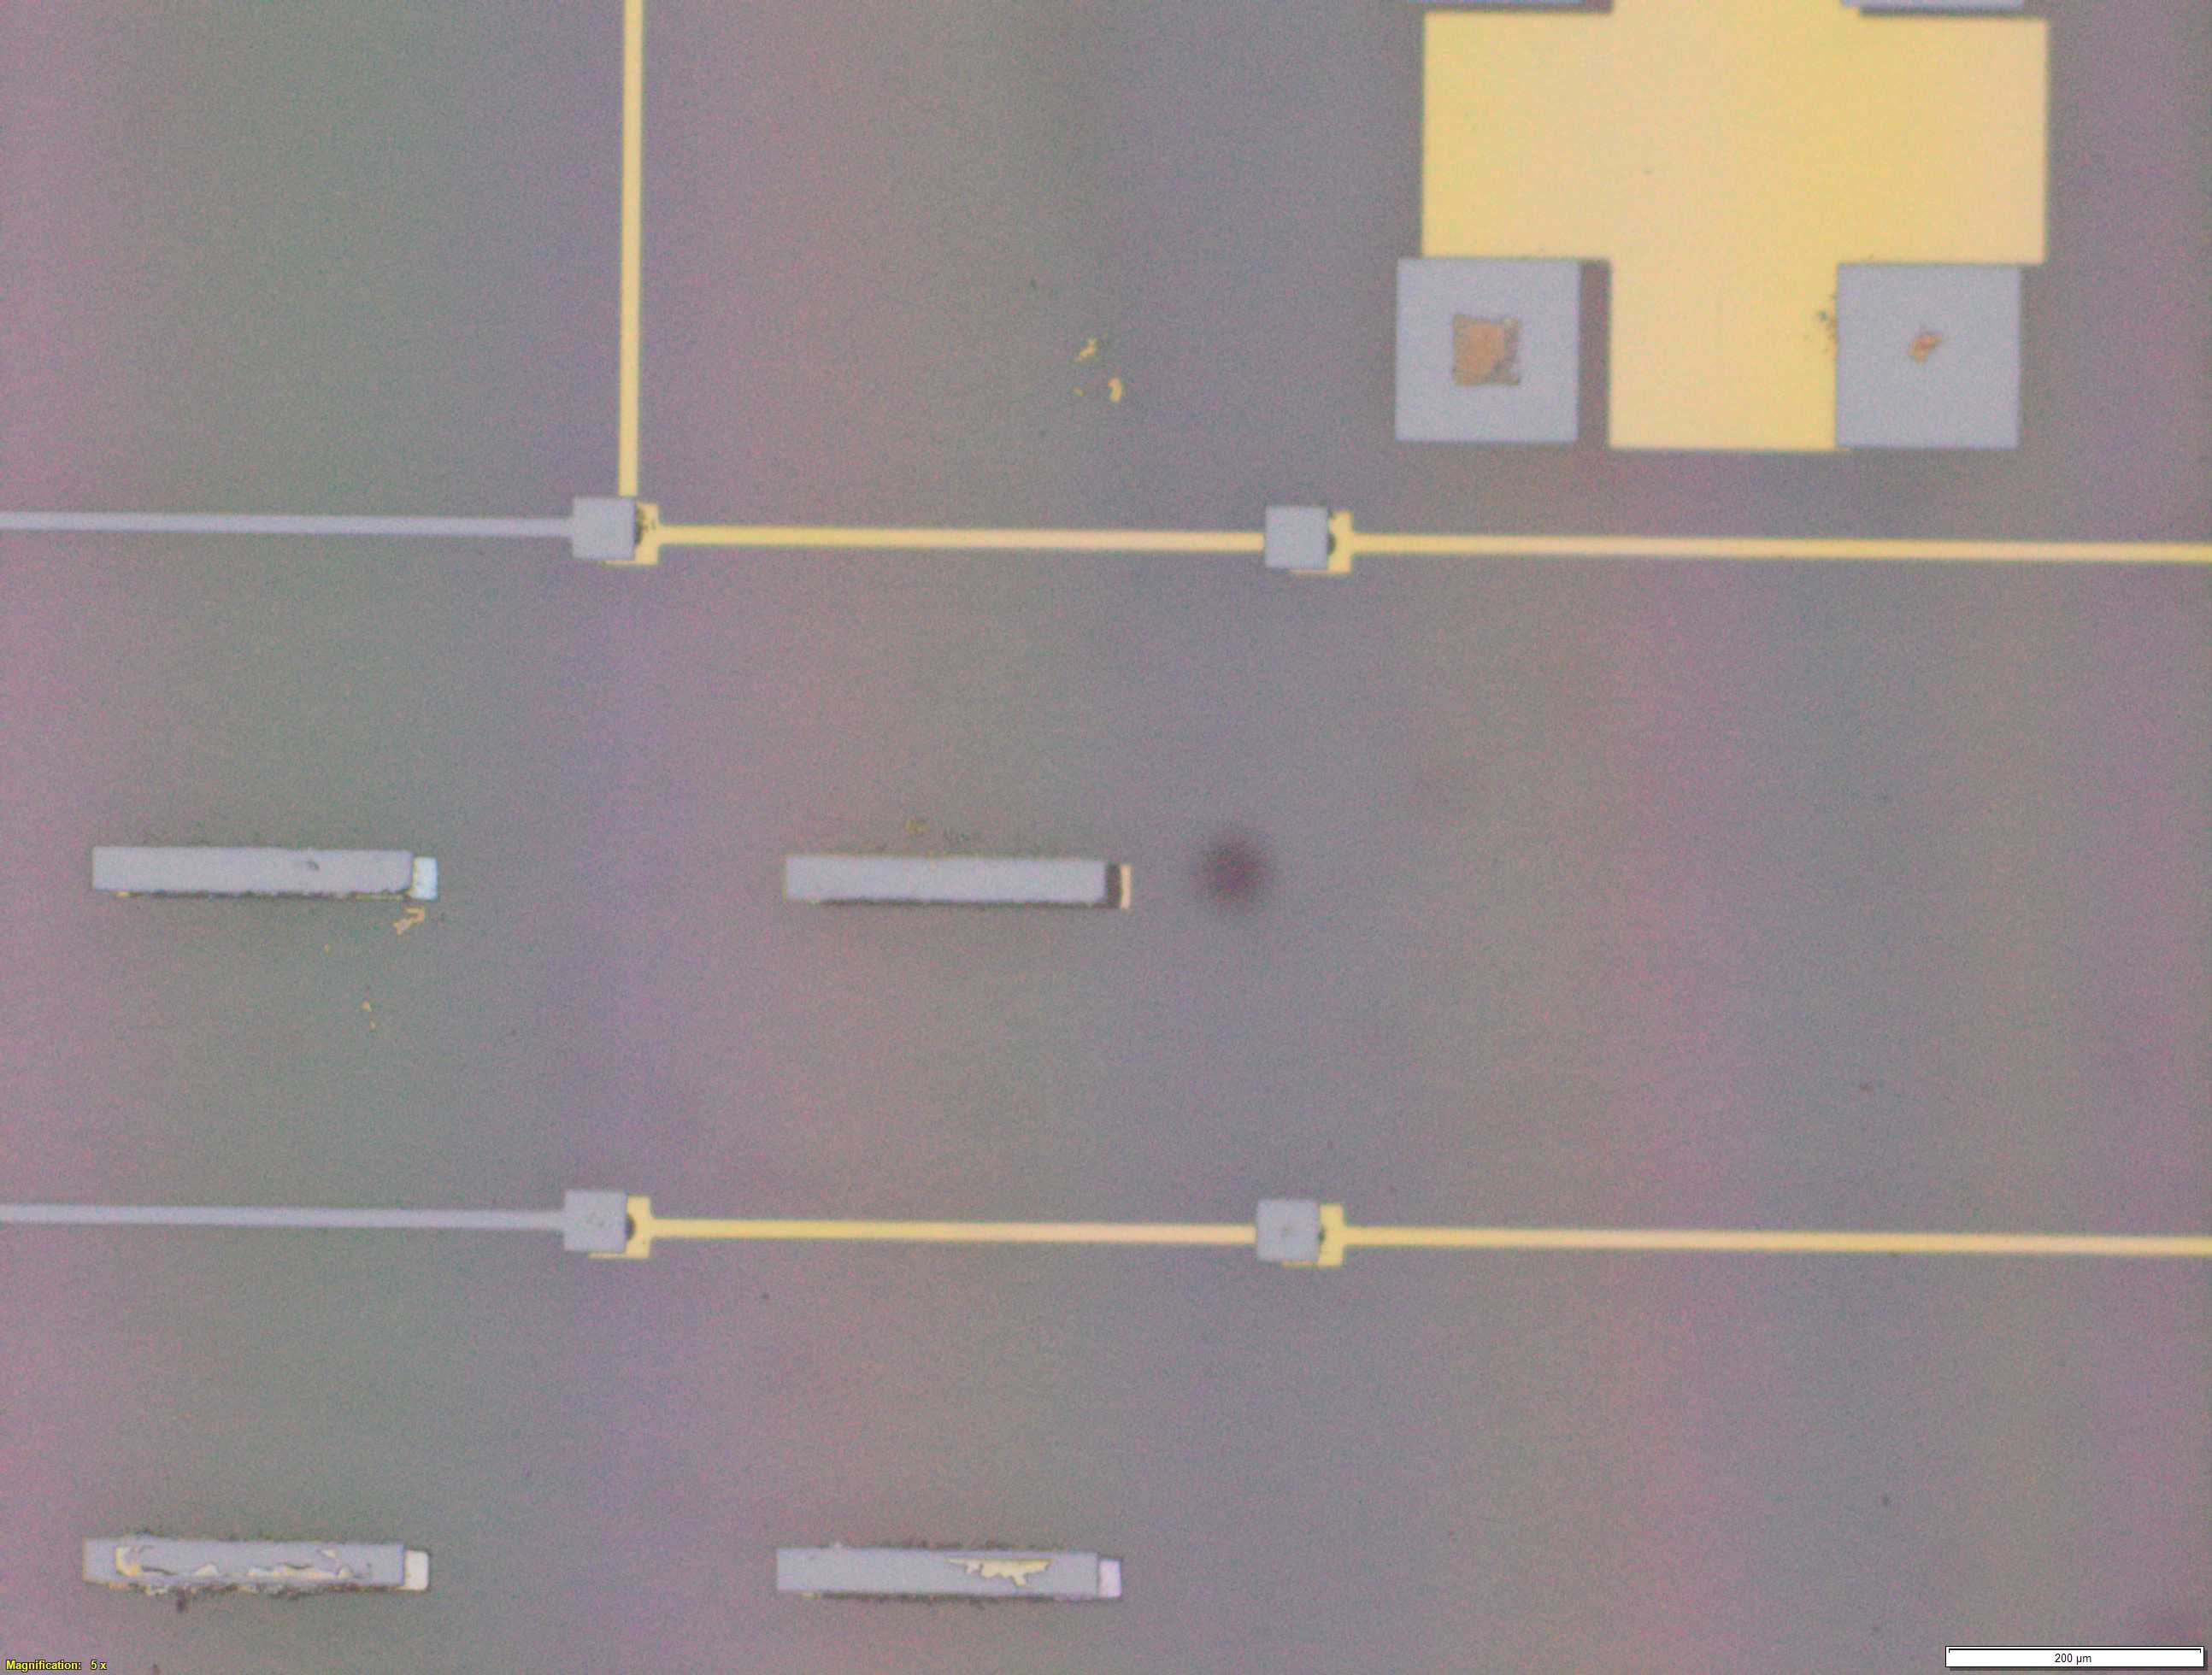
\includegraphics[width=0.22\textwidth]{Main/Ch2/TR.png} \\
    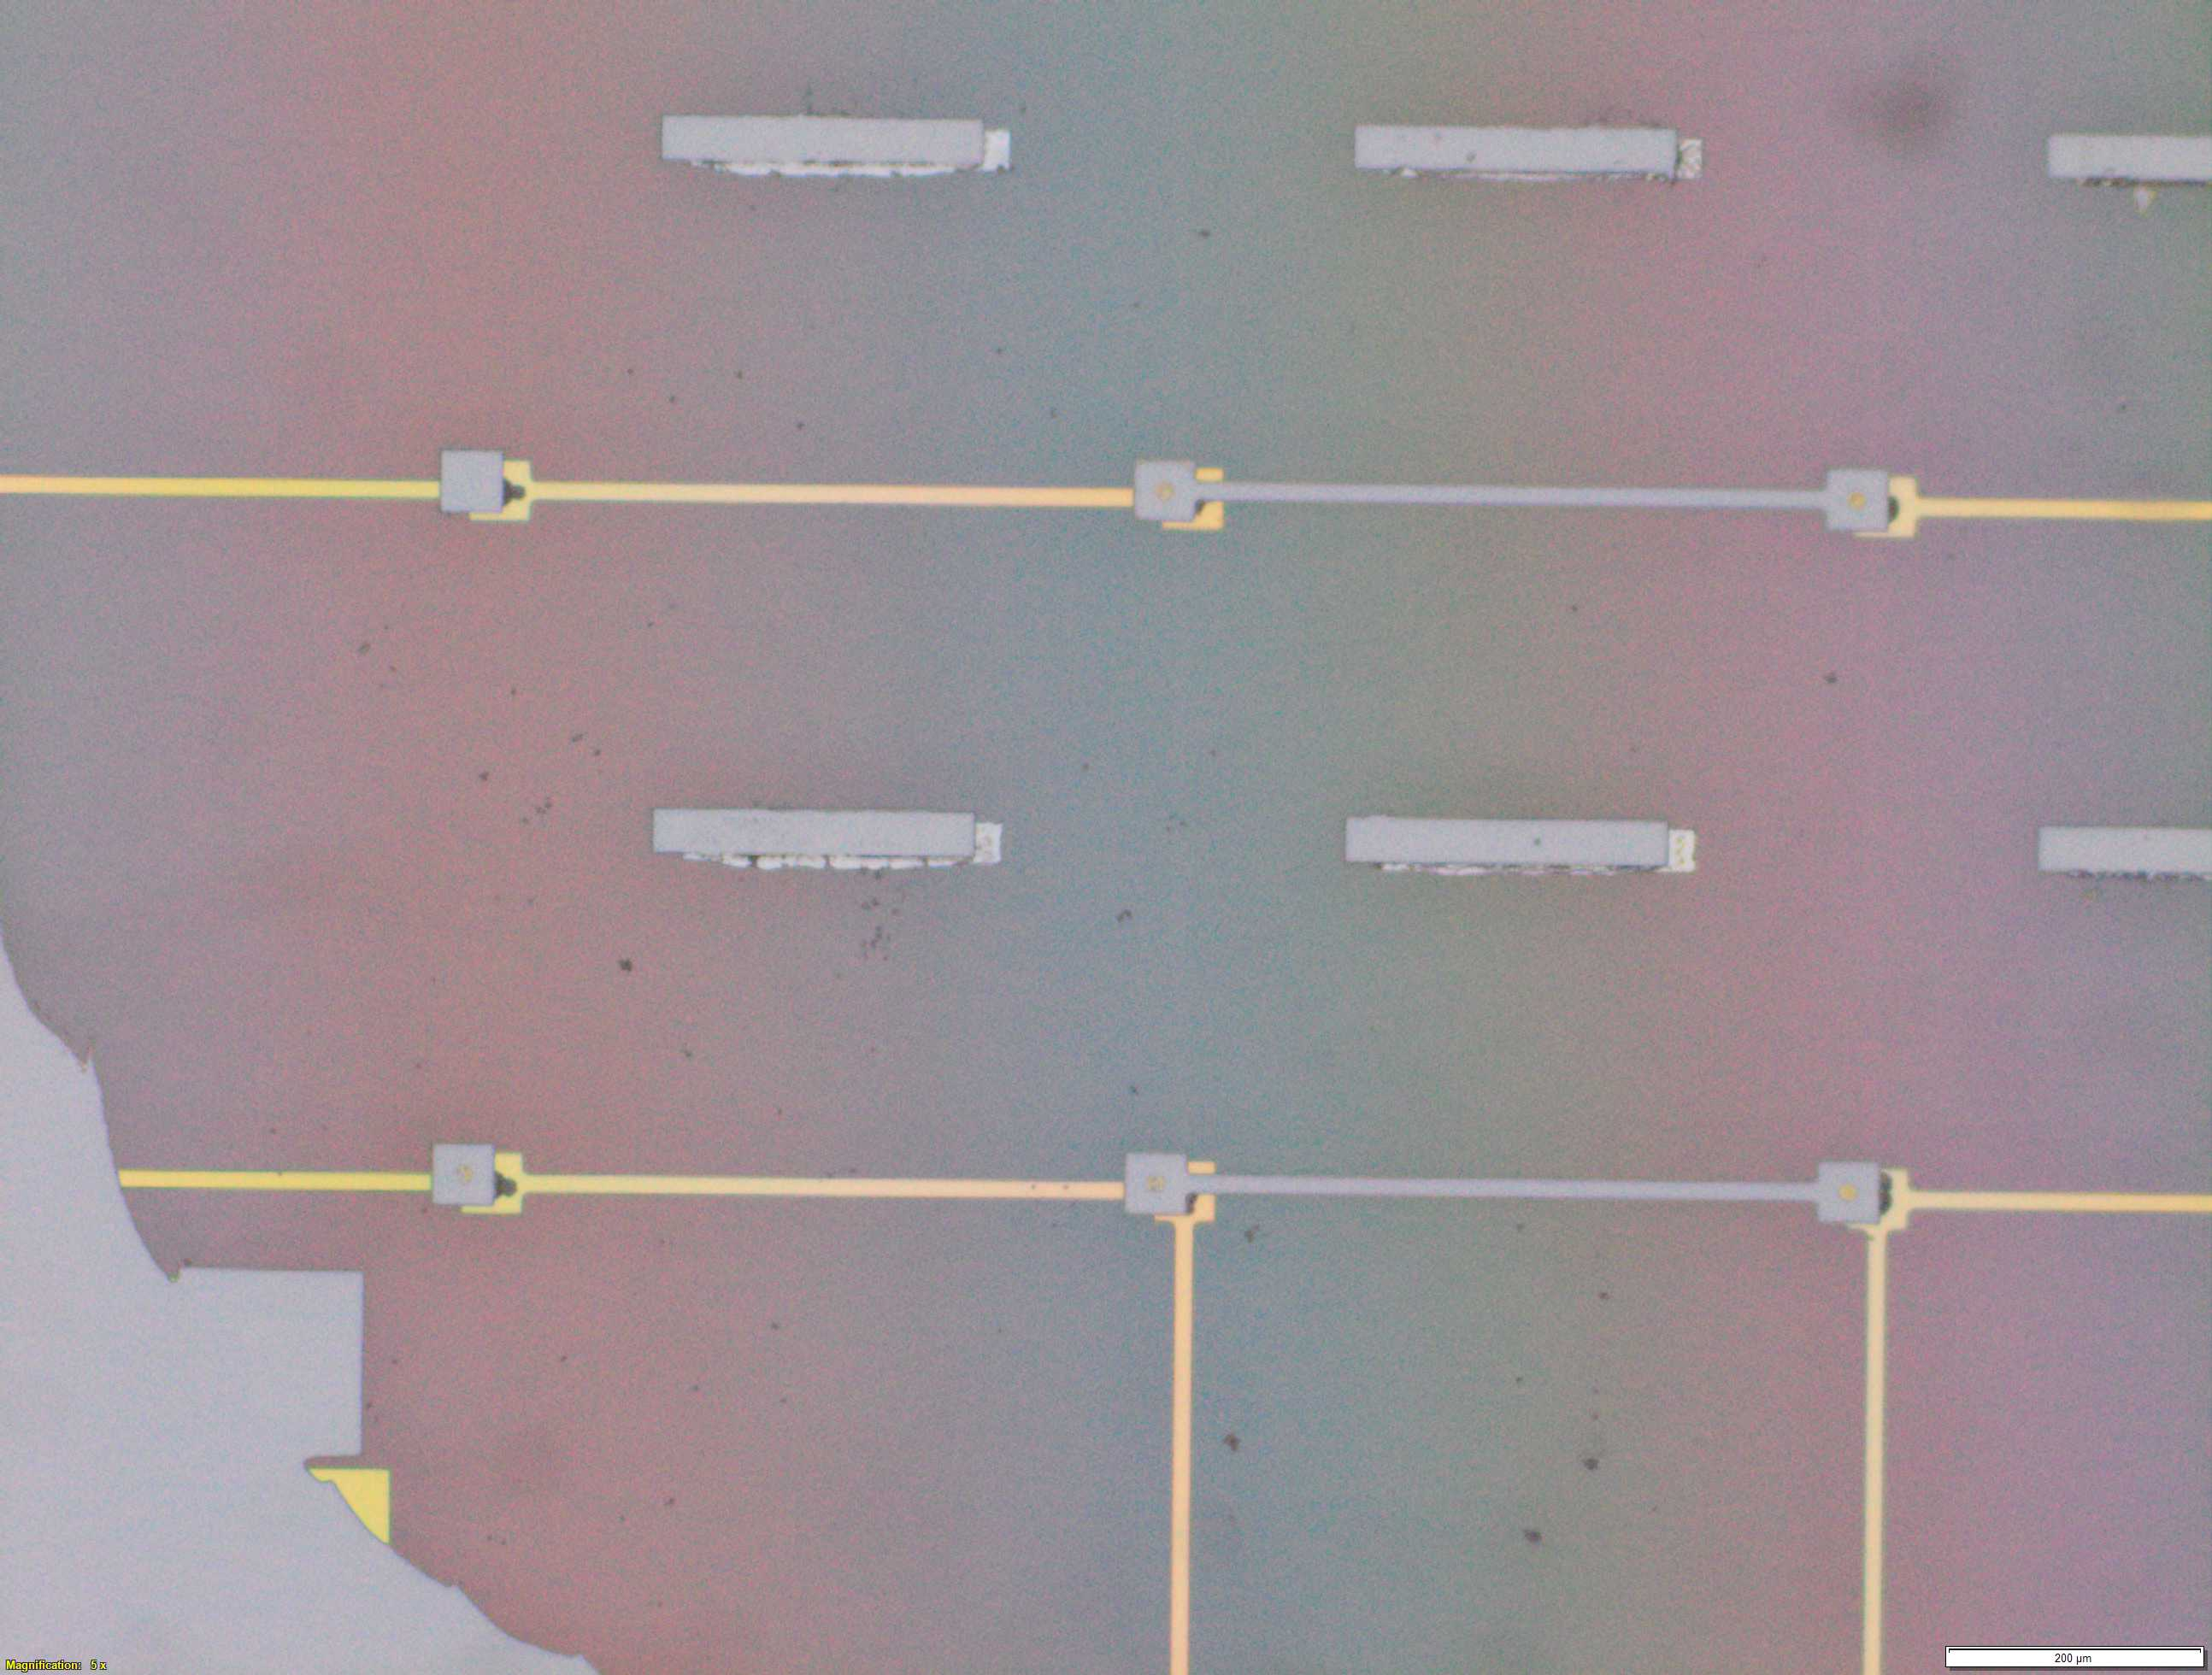
\includegraphics[width=0.22\textwidth]{Main/Ch2/BL.png}
    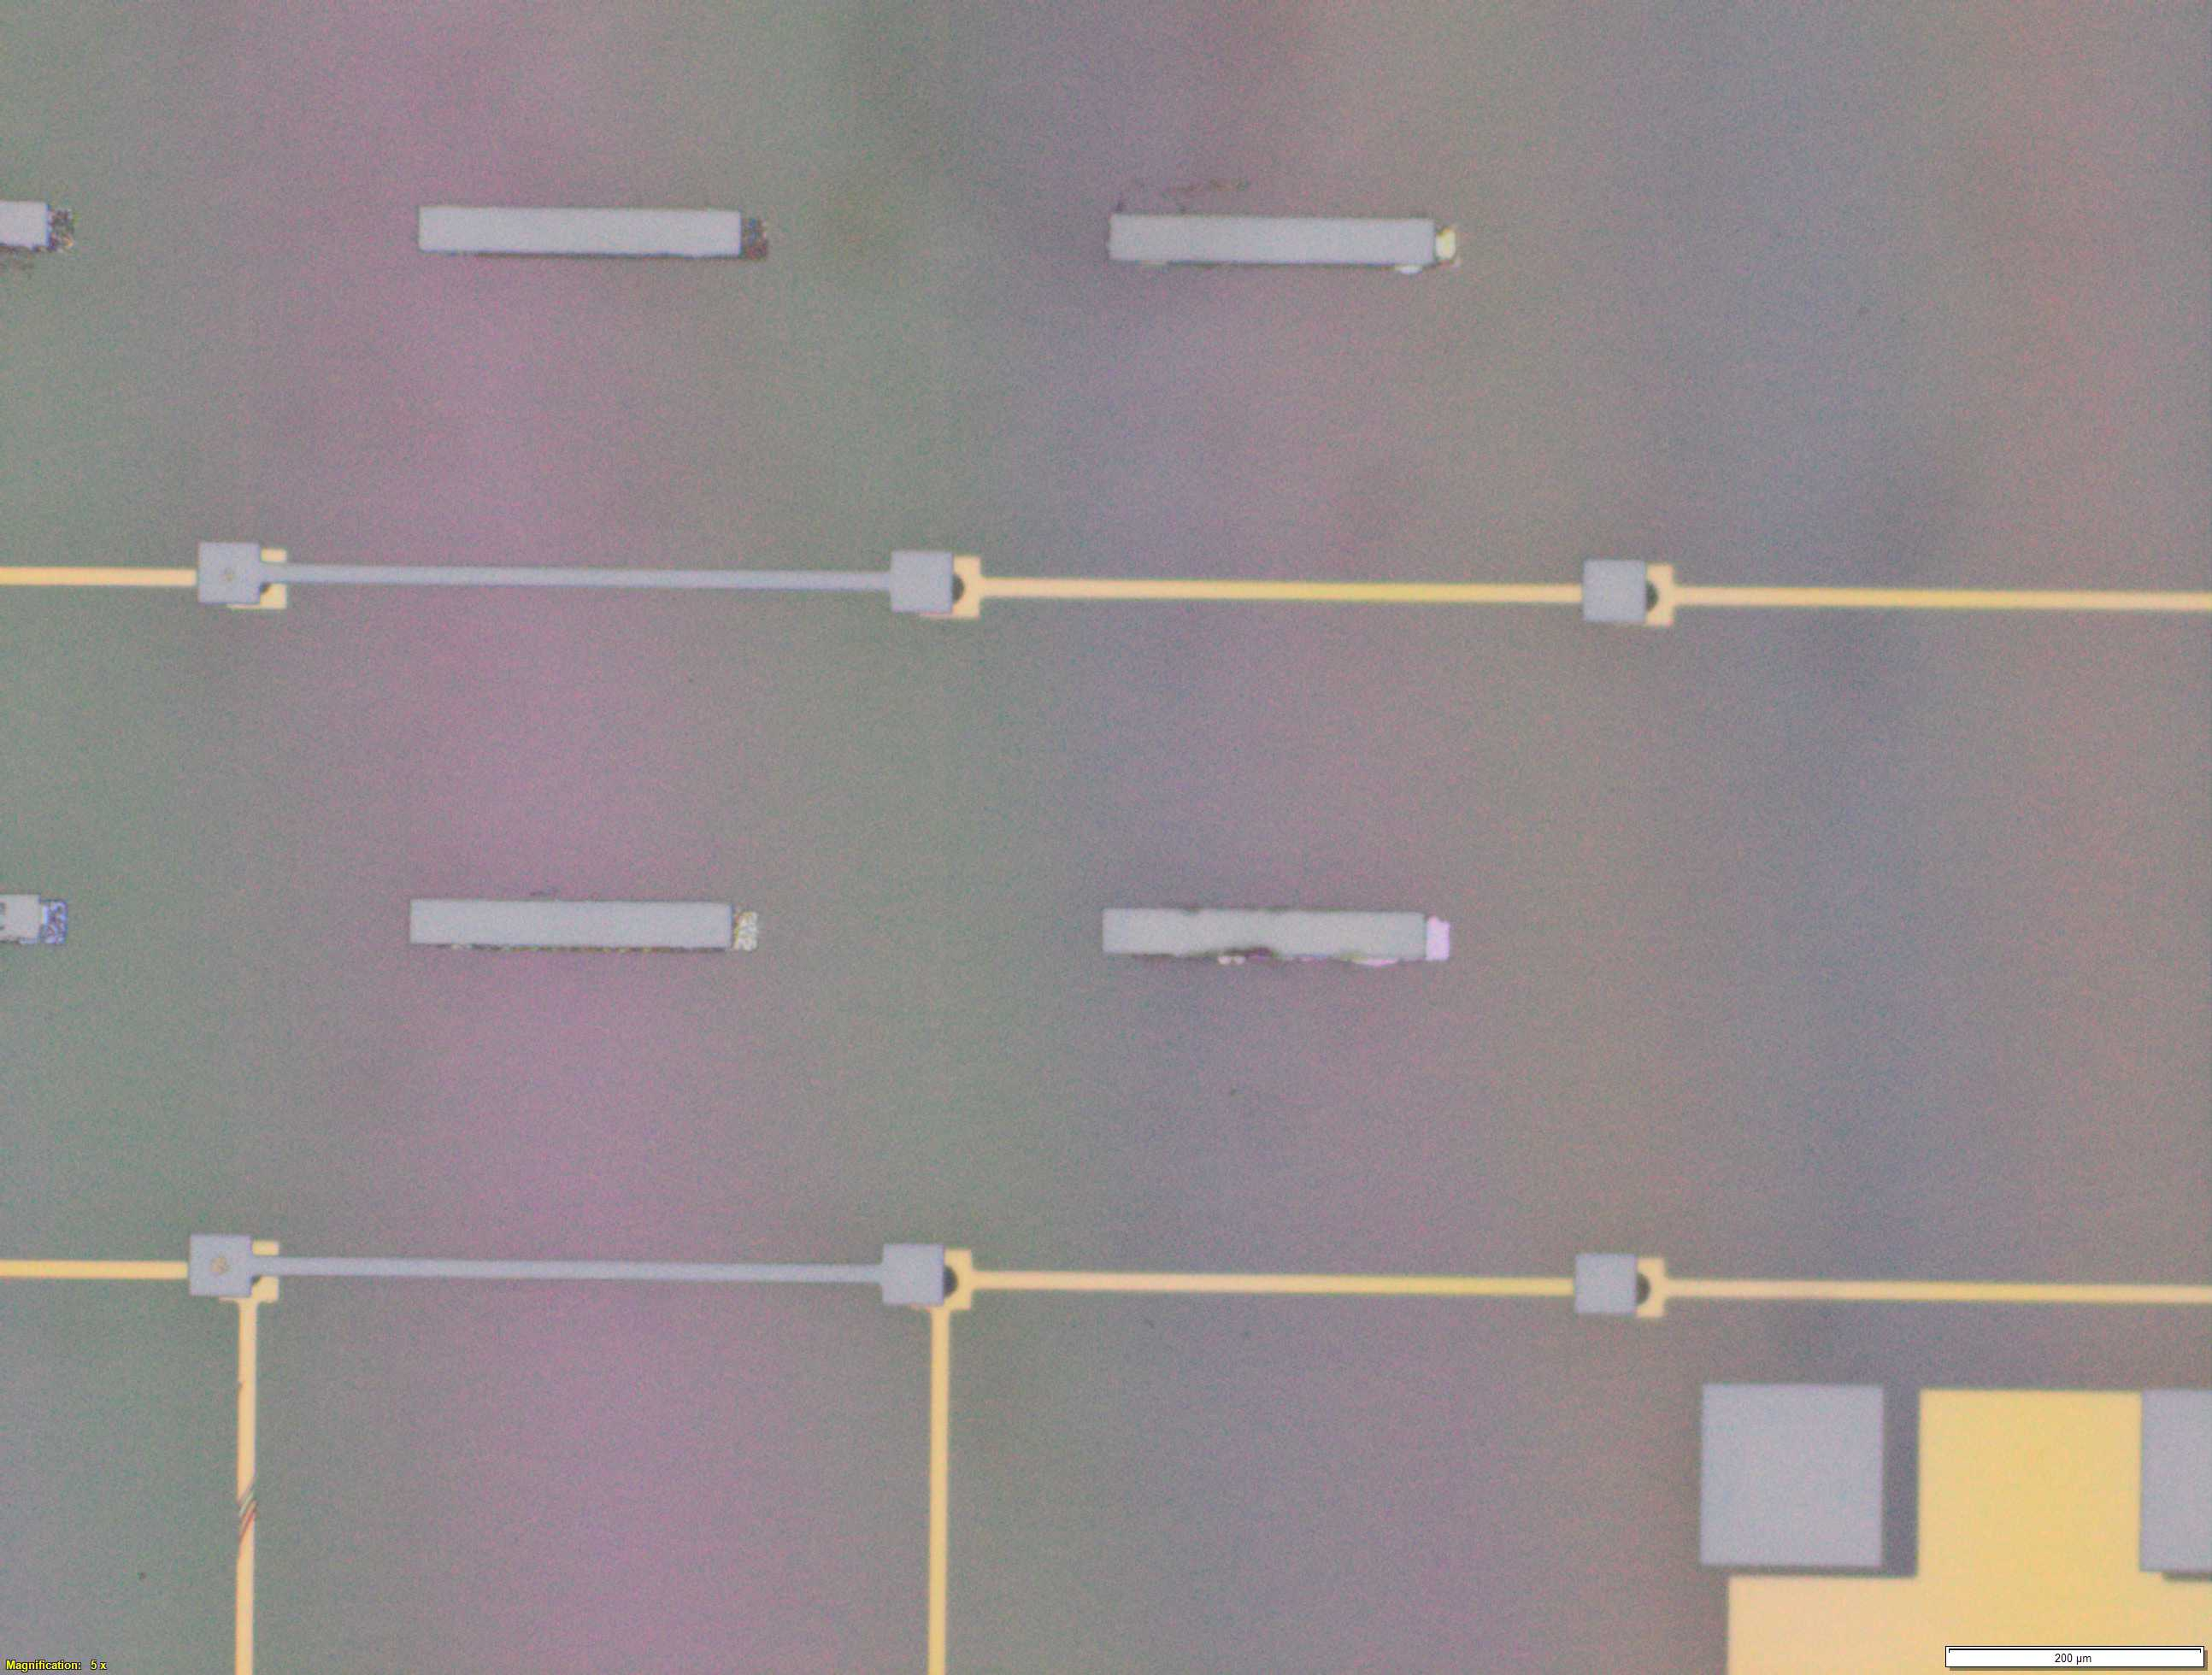
\includegraphics[width=0.22\textwidth]{Main/Ch2/BR.png}
    \caption{Microscope images of diebonded sample. The internal smaller circles seen are a diameter of $42 \um$ the larger circles are the indium spreading}
    \label{fig:microscopeIndium}
    \vspace{0.5cm}
\end{wrapfigure}

\newpage
\subsection{Thermal Simulations}

Thermal simulations were conducted because there were some bonding failures seen in the samples. As can be seen from SEM images and Energy-dispersive X-ray spectroscopy (EDX or EDS) the indium does not always appropriately wet onto the other substrate being bonded onto this is seen in the SEM images in figure \ref{fig:SEM_indium_2} and EDX images in figure \ref{fig:EDX_indium_2}. There can be various reasons why indium does not wet onto a surface during diebonding. One reason could be the presence of surface contaminants such as oxides or oils, which can prevent the indium from bonding to the surface. Another reason could be an insufficient amount of heat or pressure during the diebonding process, which can cause the indium to not properly wet onto the surface. Additionally, the surface energy of the substrate can also affect the ability of indium to wet onto the surface during diebonding.

To explore further a lack of heat, thermal simulations were conducted to identify if a process change in the diebonding preocess was required. Thermal simulations were done in MATLAB with the following code in  \hyperref[sec:ThermalSimulationCode]{Appendix B}.


\begin{wrapfigure}{L}{0.45\textwidth}
    \centering
    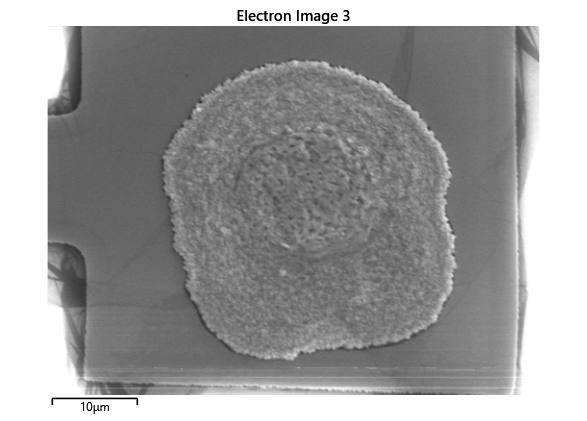
\includegraphics[width=0.1\textwidth]{Main/Ch2/extracted/SEM/In-EP-EDx_TBP-01-A1-s1_media_image.png}
    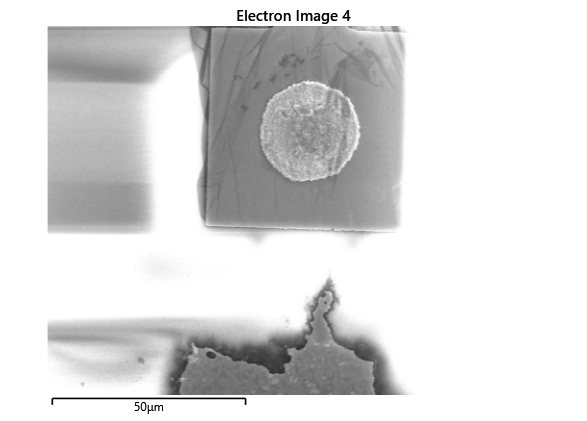
\includegraphics[width=0.1\textwidth]{Main/Ch2/extracted/SEM/In-EP-EDx_TBP-01-A1-s2_media_image.png}
    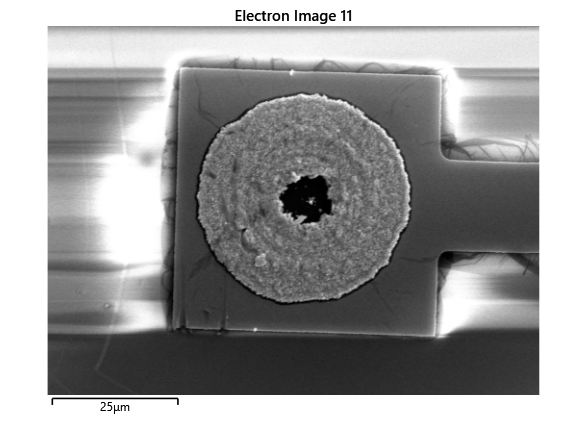
\includegraphics[width=0.1\textwidth]{Main/Ch2/extracted/SEM/In-EP-EDx_TBP-01-A2-s1_media_image.png}
    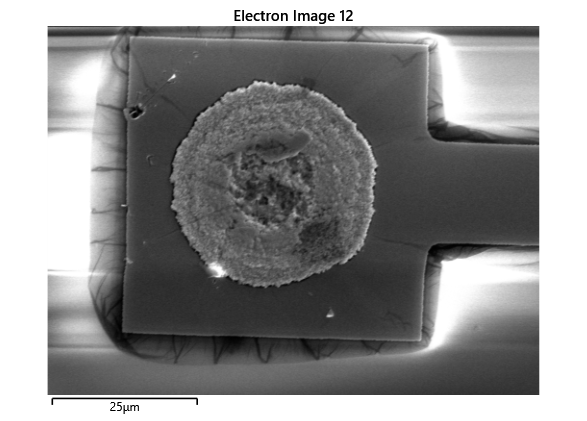
\includegraphics[width=0.1\textwidth]{Main/Ch2/extracted/SEM/In-EP-EDx_TBP-01-A2-s2_media_image.png}
    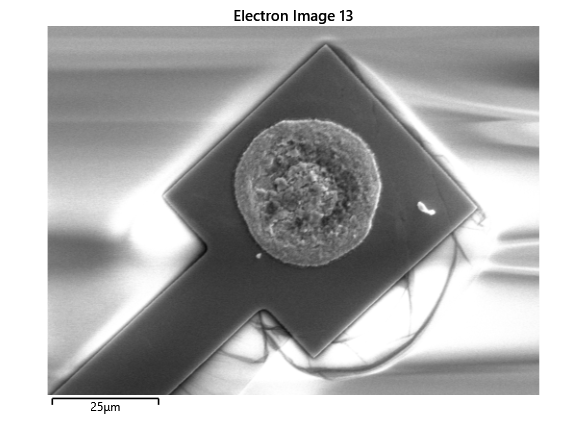
\includegraphics[width=0.1\textwidth]{Main/Ch2/extracted/SEM/In-EP-EDx_TBP-01-B2-s1_media_image.png}
    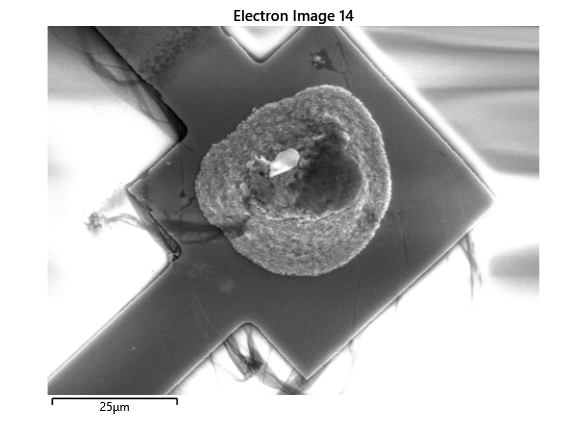
\includegraphics[width=0.1\textwidth]{Main/Ch2/extracted/SEM/In-EP-EDx_TBP-01-B2-s2_media_image.png}
    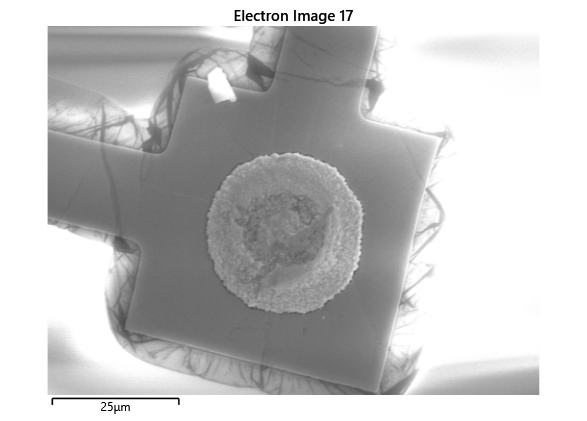
\includegraphics[width=0.1\textwidth]{Main/Ch2/extracted/SEM/In-EP-EDx_TBP-02-A1-s1_media_image.png}
    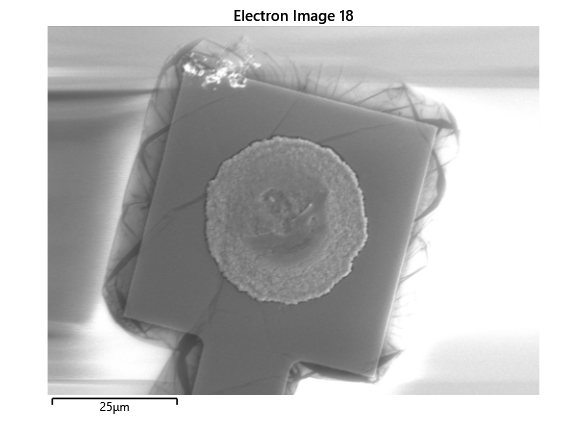
\includegraphics[width=0.1\textwidth]{Main/Ch2/extracted/SEM/In-EP-EDx_TBP-02-A1-s2_media_image.png}
    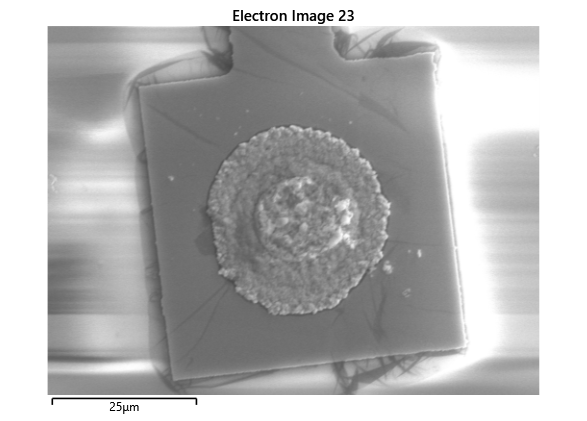
\includegraphics[width=0.1\textwidth]{Main/Ch2/extracted/SEM/In-EP-EDx_TBP-02-A2-s1_media_image.png}
    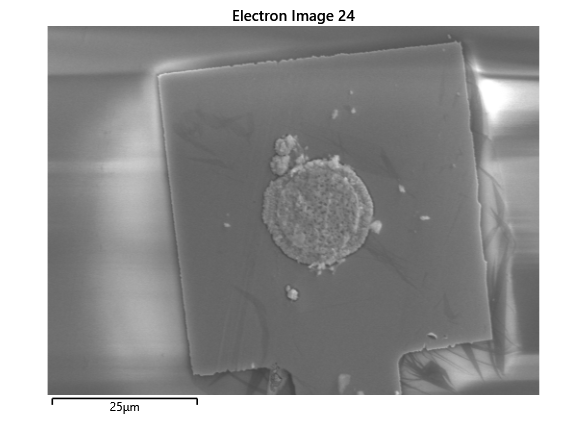
\includegraphics[width=0.1\textwidth]{Main/Ch2/extracted/SEM/In-EP-EDx_TBP-02-A2-s2_media_image.png}
    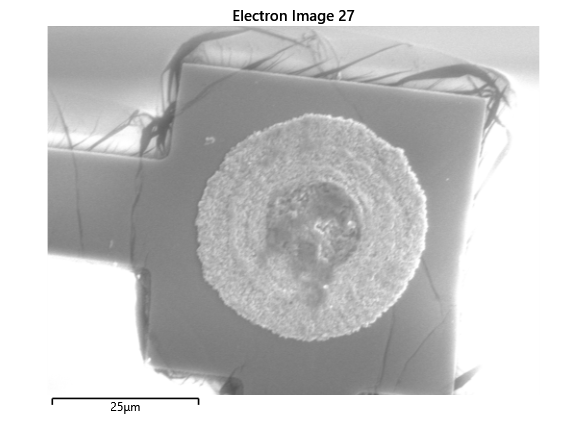
\includegraphics[width=0.1\textwidth]{Main/Ch2/extracted/SEM/In-EP-EDx_TBP-02-B2-s1_media_image.png}
    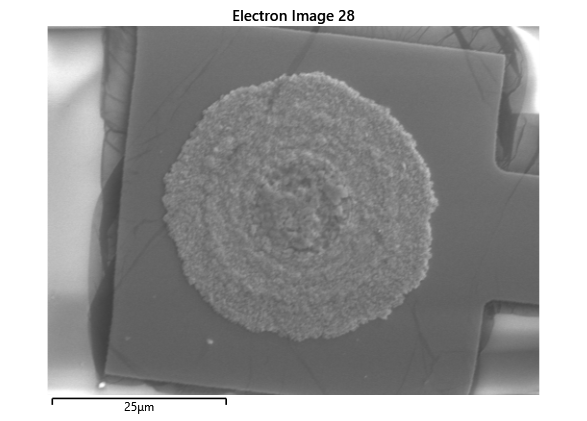
\includegraphics[width=0.1\textwidth]{Main/Ch2/extracted/SEM/In-EP-EDx_TBP-02-B2-s2_media_image.png}
    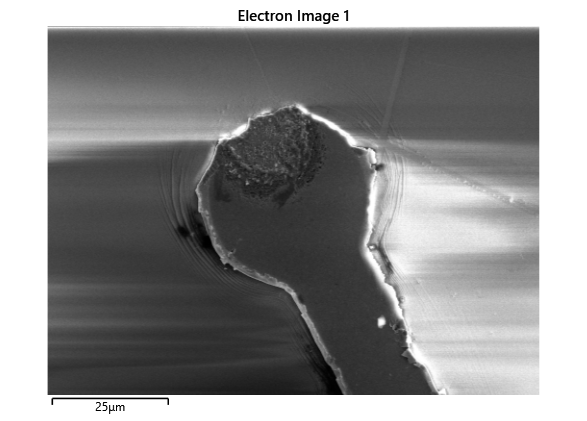
\includegraphics[width=0.1\textwidth]{Main/Ch2/extracted/SEM/In-EP-EDx_TLED-01-A1-s1_media_image.png}
    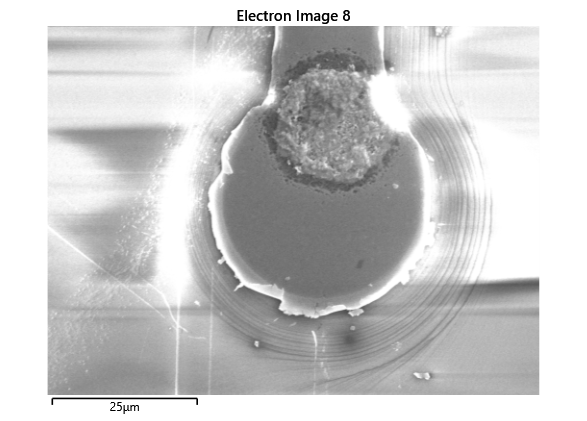
\includegraphics[width=0.1\textwidth]{Main/Ch2/extracted/SEM/In-EP-EDx_TLED-01-A1-s2_media_image.png}
    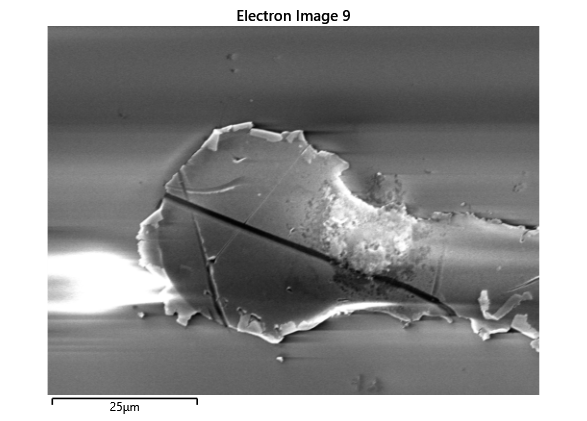
\includegraphics[width=0.1\textwidth]{Main/Ch2/extracted/SEM/In-EP-EDx_TLED-01-A2-s1_media_image.png}
    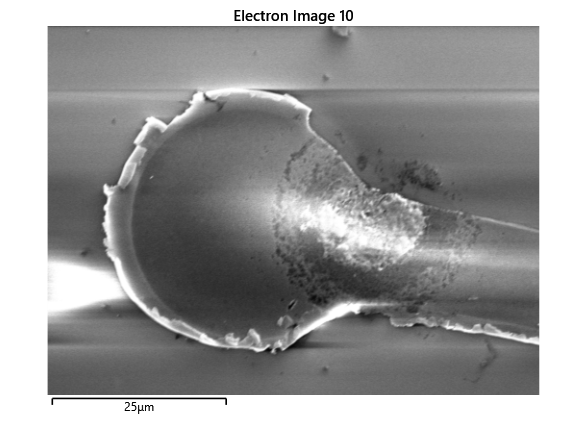
\includegraphics[width=0.1\textwidth]{Main/Ch2/extracted/SEM/In-EP-EDx_TLED-01-A2-s2_media_image.png}
    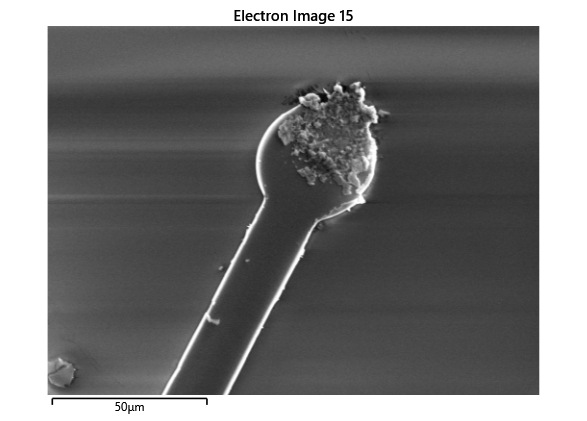
\includegraphics[width=0.1\textwidth]{Main/Ch2/extracted/SEM/In-EP-EDx_TLED-01-B2-s1_media_image.png}
    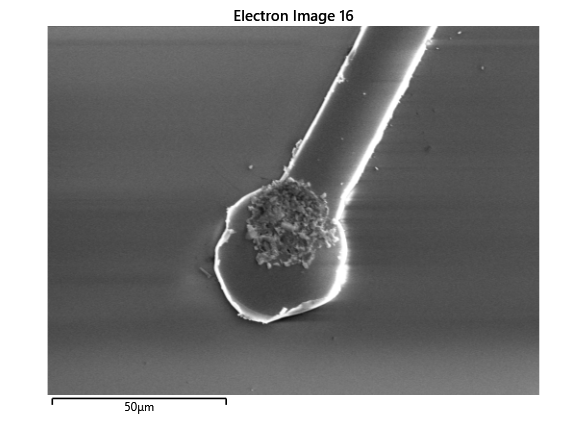
\includegraphics[width=0.1\textwidth]{Main/Ch2/extracted/SEM/In-EP-EDx_TLED-01-B2-s2_media_image.png}
    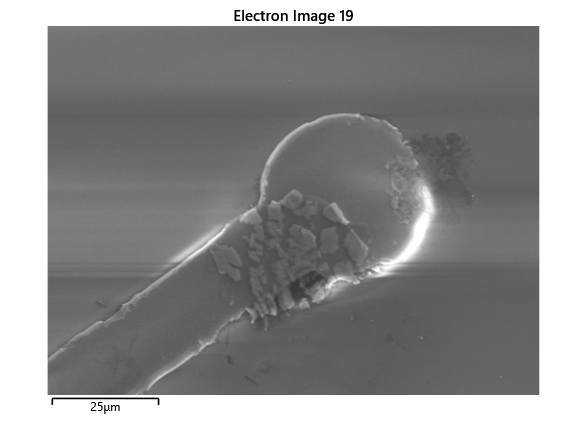
\includegraphics[width=0.1\textwidth]{Main/Ch2/extracted/SEM/In-EP-EDx_TLED-02-A1-s1_media_image.png}
    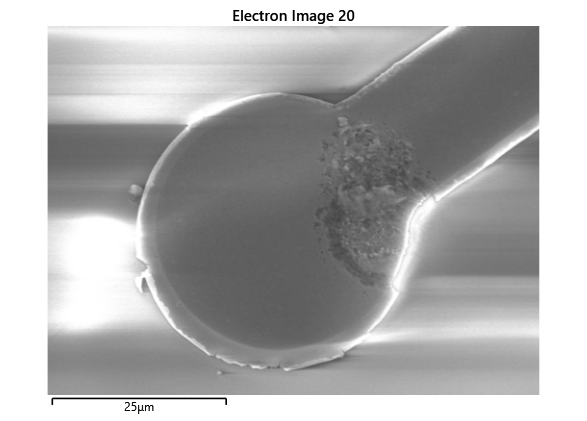
\includegraphics[width=0.1\textwidth]{Main/Ch2/extracted/SEM/In-EP-EDx_TLED-02-A1-s2_media_image.png}
    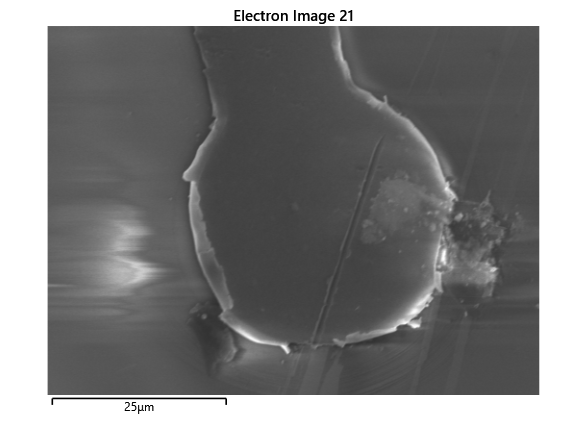
\includegraphics[width=0.1\textwidth]{Main/Ch2/extracted/SEM/In-EP-EDx_TLED-02-A2-s1_media_image.png}
    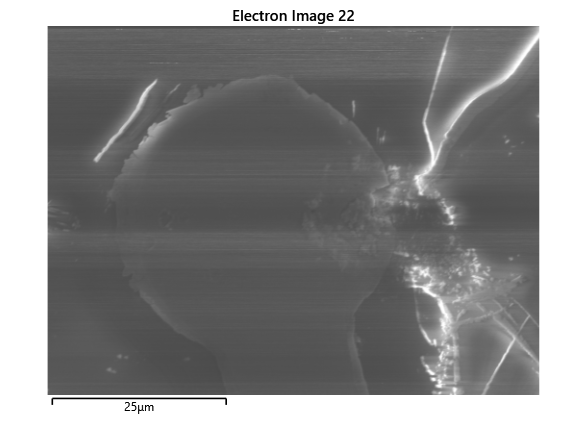
\includegraphics[width=0.1\textwidth]{Main/Ch2/extracted/SEM/In-EP-EDx_TLED-02-A2-s2_media_image.png}
    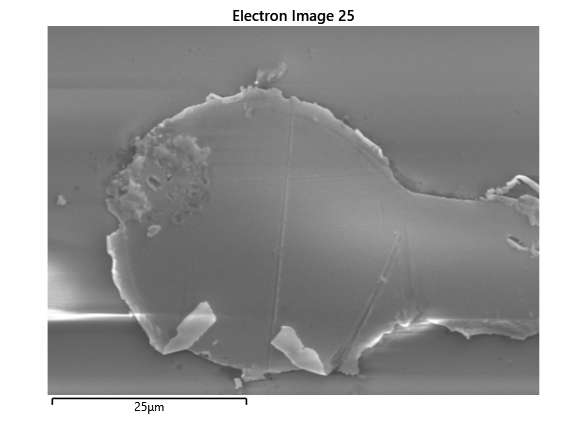
\includegraphics[width=0.1\textwidth]{Main/Ch2/extracted/SEM/In-EP-EDx_TLED-02-B2-s1_media_image.png}
    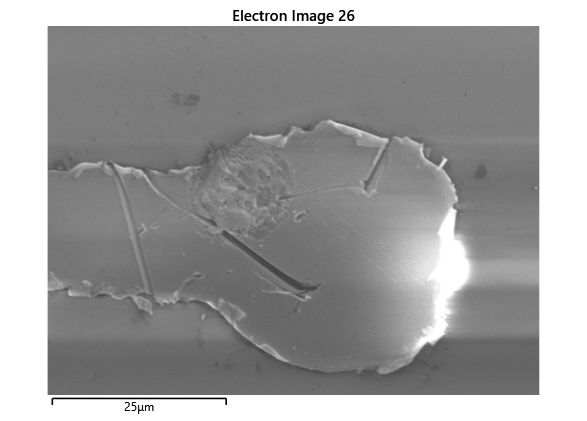
\includegraphics[width=0.1\textwidth]{Main/Ch2/extracted/SEM/In-EP-EDx_TLED-02-B2-s2_media_image.png}
    \caption{SEM Images of bonds}
    \label{fig:SEM_indium_2}
    \vspace{0.5cm}
\end{wrapfigure}


\begin{wrapfigure}{R}{0.45\textwidth}
    \centering
    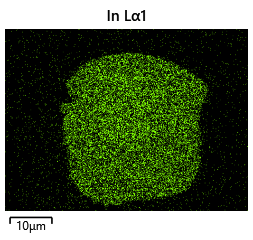
\includegraphics[width=0.1\textwidth]{Main/Ch2/extracted/Indium/In-EP-EDx_TBP-01-A1-s1_media_image7.png}
    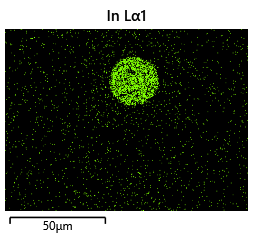
\includegraphics[width=0.1\textwidth]{Main/Ch2/extracted/Indium/In-EP-EDx_TBP-01-A1-s2_media_image7.png}
    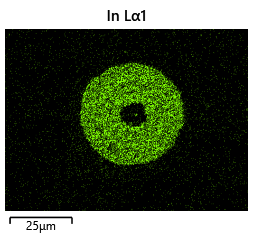
\includegraphics[width=0.1\textwidth]{Main/Ch2/extracted/Indium/In-EP-EDx_TBP-01-A2-s1_media_image7.png}
    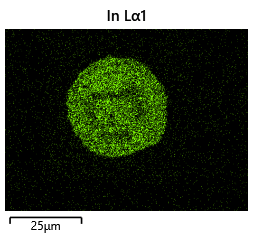
\includegraphics[width=0.1\textwidth]{Main/Ch2/extracted/Indium/In-EP-EDx_TBP-01-A2-s2_media_image7.png}
    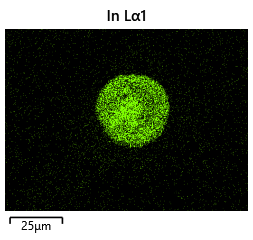
\includegraphics[width=0.1\textwidth]{Main/Ch2/extracted/Indium/In-EP-EDx_TBP-01-B2-s1_media_image7.png}
    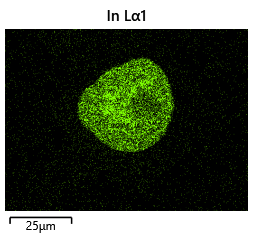
\includegraphics[width=0.1\textwidth]{Main/Ch2/extracted/Indium/In-EP-EDx_TBP-01-B2-s2_media_image7.png}
    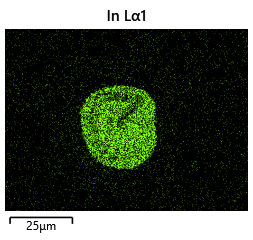
\includegraphics[width=0.1\textwidth]{Main/Ch2/extracted/Indium/In-EP-EDx_TBP-02-A1-s1_media_image7.png}
    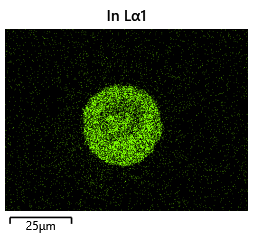
\includegraphics[width=0.1\textwidth]{Main/Ch2/extracted/Indium/In-EP-EDx_TBP-02-A1-s2_media_image7.png}
    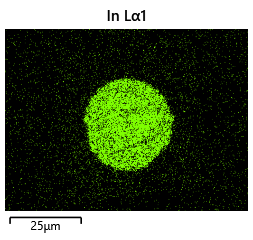
\includegraphics[width=0.1\textwidth]{Main/Ch2/extracted/Indium/In-EP-EDx_TBP-02-A2-s1_media_image7.png}
    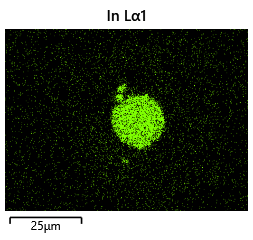
\includegraphics[width=0.1\textwidth]{Main/Ch2/extracted/Indium/In-EP-EDx_TBP-02-A2-s2_media_image7.png}
    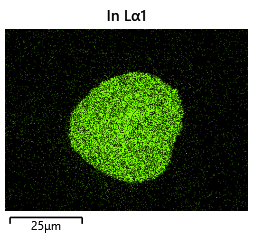
\includegraphics[width=0.1\textwidth]{Main/Ch2/extracted/Indium/In-EP-EDx_TBP-02-B2-s1_media_image7.png}
    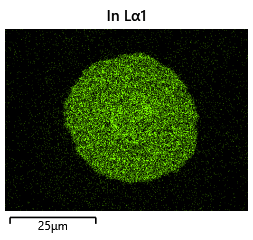
\includegraphics[width=0.1\textwidth]{Main/Ch2/extracted/Indium/In-EP-EDx_TBP-02-B2-s2_media_image7.png}
    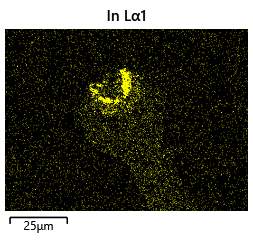
\includegraphics[width=0.1\textwidth]{Main/Ch2/extracted/Indium/In-EP-EDx_TLED-01-A1-s1_media_image7.png}
    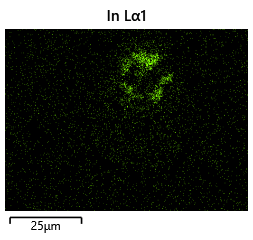
\includegraphics[width=0.1\textwidth]{Main/Ch2/extracted/Indium/In-EP-EDx_TLED-01-A1-s2_media_image7.png}
    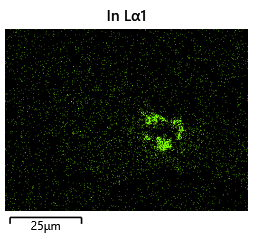
\includegraphics[width=0.1\textwidth]{Main/Ch2/extracted/Indium/In-EP-EDx_TLED-01-A2-s1_media_image7.png}
    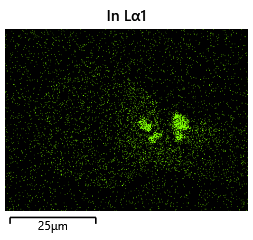
\includegraphics[width=0.1\textwidth]{Main/Ch2/extracted/Indium/In-EP-EDx_TLED-01-A2-s2_media_image7.png}
    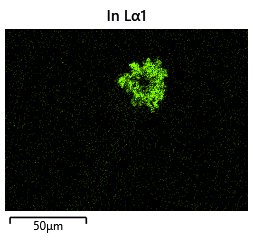
\includegraphics[width=0.1\textwidth]{Main/Ch2/extracted/Indium/In-EP-EDx_TLED-01-B2-s1_media_image7.png}
    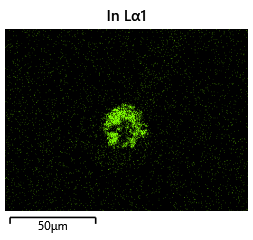
\includegraphics[width=0.1\textwidth]{Main/Ch2/extracted/Indium/In-EP-EDx_TLED-01-B2-s2_media_image7.png}
    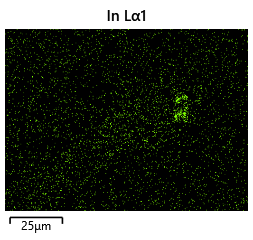
\includegraphics[width=0.1\textwidth]{Main/Ch2/extracted/Indium/In-EP-EDx_TLED-02-A1-s1_media_image7.png}
    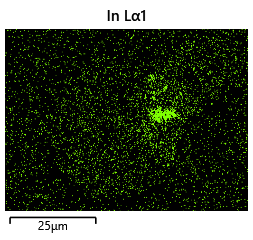
\includegraphics[width=0.1\textwidth]{Main/Ch2/extracted/Indium/In-EP-EDx_TLED-02-A1-s2_media_image7.png}
    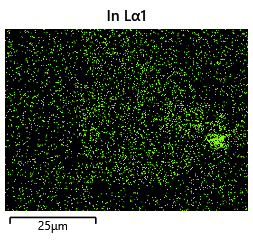
\includegraphics[width=0.1\textwidth]{Main/Ch2/extracted/Indium/In-EP-EDx_TLED-02-A2-s1_media_image7.png}
    \includegraphics[width=0.1\textwidth]{Main/Ch2/extracted/Indium/In-EP-EDx_TLED-02-A2-s2_media_image7.png}
    \includegraphics[width=0.1\textwidth]{Main/Ch2/extracted/Indium/In-EP-EDx_TLED-02-B2-s1_media_image7.png}
    \includegraphics[width=0.1\textwidth]{Main/Ch2/extracted/Indium/In-EP-EDx_TLED-02-B2-s2_media_image7.png}
    \caption{EDX Images of bonds}
    \label{fig:EDX_indium_2}
\end{wrapfigure}


The results from the thermal simulations as seen in figure \ref{fig:thermal_simulations} in MATLAB were that there was more than sufficient time and heat to melt and wet the indium onto the opposing surface. As a result the lack of wetting was likely a result of one of the other issues (contaminants from the flip-chip process or some failure in the surface energies).
Both of the other issues are quite possible as during the process the substrate that is bonding onto the substrate with indium on the surface is face down on the `diebonder' which is a unclean surface that also does not have the appropriate surface energies and could dissapate the surface energy generated during the plasma cleaning process.
% TODO Verify statement about suface energy

It can be seen from the thermal simulations that the time taken for the indium to reach temperature is well within $0.3 \unit{\second}$ whereas the bonding recipe calls for the sample to sit at $250 \dC$ for $5 \unit{\minute}$. This is well within 2 orders of magnitude of time for the sample to reach temperature, as such it would be safe to assume that heat/temperature or lack thereof is not the causal source of failure.


\begin{wrapfigure}{L}{0.5\textwidth}
    \includegraphics[width=0.21\textwidth]{Main/Ch2/heat/001.png}
    \includegraphics[width=0.21\textwidth]{Main/Ch2/heat/002.png}
    \includegraphics[width=0.21\textwidth]{Main/Ch2/heat/008.png}
    \includegraphics[width=0.21\textwidth]{Main/Ch2/heat/020.png}
    \caption{Thermal simulation results. Temperature scale is ranged from $25 \dC$ to $250 \dC$}
    \label{fig:thermal_simulations}
\end{wrapfigure}


\subsection{Conformation to Theory}
Conformed to theory when the bonding would spread according to the calculated volume

\subsection{Development of a Repeatable Process}
% Adding anchors